\documentclass[10pt]{article}
\usepackage{fontspec}
\usepackage{polyglossia}
\setdefaultlanguage{french}
\usepackage[a4paper,margin=2.5cm]{geometry}
\usepackage{url,hyperref}
\usepackage{siunitx}
\usepackage{schemabloc}
\usepackage{listings}
\usepackage{auto-pst-pdf}
\usepackage{pst-circ}
\usepackage{soul}
\usepackage{verbatim}
\usepackage{lmodern}
\usepackage{tikz}
\usepackage[european,cuteinductors,siunitx]{circuitikz}
\usepackage{xunicode,xltxtra}
\usepackage{graphicx}
\usepackage{amsmath}
\usepackage{minted}
\usepackage{multicol}
\title{
\includegraphics{inp-enseeiht} \\ ~ \\ ~ \\ ~ \\ ~ \\BE Lignes de transmissions}
\author{Ken Hasselmann, Guilhem Saurel}
\date{\today}
\begin{document}

 \begin{titlepage}
  \maketitle
  \tableofcontents
 \end{titlepage}

 \part{Ligne de transmission}
  \section{Mise en œuvre d’une simulation Paramètre S}
   Valeur normalisée de l’impédance : $z_L=\cfrac{Z_L}{Z_0}=\cfrac{80 + j 5 \cdot 10^{-9} \cdot 2 \pi 2 \cdot 10^9}{50} = 1.6+i1.26$

   Coefficient de réflexion correspondant : $\Gamma = \cfrac{z_L-1}{z_L+1}=0.38+i0.30$

   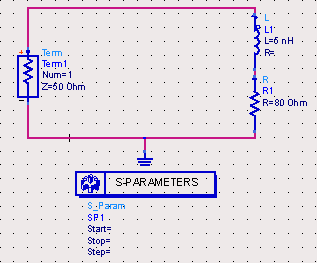
\includegraphics{I2_a_circuit.PNG}

   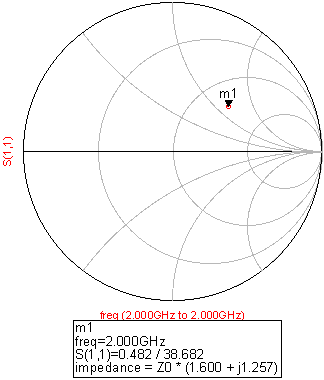
\includegraphics{I2_a_smith.PNG}

   Lorsque l’on ajoute une ligne de transmission entre la source et la charge, on obtient une impédance ramenée au niveau du port d’entrée de $z_E = \cfrac{z_L +j \tan{\beta d}}{1 + j z_L \tan{\beta d}}=\cfrac{z_L +j \tan{E}}{1 + j z_L \tan{E}}$

   Coefficient de réflexion correspondant : $\Gamma=\cfrac{z_E-1}{z_E+1}$

   Dans le cas particulier d’une ligne quart d’onde, ceci donne $-0.38-i0.30$

   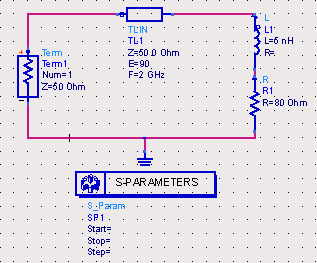
\includegraphics[width=8cm]{I2_b_circuit.PNG}

   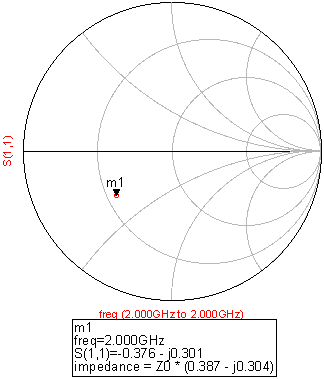
\includegraphics[width=8cm]{I2_b_smith.PNG}

 \part{Annexes}
  Voici le fichier Scilab contenant tous les calculs :
  %\inputminted{scilab}{calculs.sci}



\end{document}
